\Exercise
\label{Ex:interpolacio2}

Considereu a $\mathbb{R}^2$ els punts $P_0=(1,2)$, $P_1=(2,5)$, $P_2=(3,7)$ i $P_3=(4,3)$ i els vectors $\overrightarrow{P_0'}=(-1,2)$ i $\overrightarrow{P_1'}=(2,-5)$


Considerant els 4 punts $P_0=(1,1)$, $P_1=(2,5)$, $P_2=(3,4)$ i $P_3=(4,2)$, i recordant que la interpolació de Béziers ens ajuda a construir un spline cúbic seguint $Q_0(t)=T\cdot M \cdot G$ on
$  T= \begin{pmatrix}t^3 & t^2 & t & 1\end{pmatrix}$, $M= \begin{pmatrix}
              -1 & 3 & -3 & 1 \\
              3 & -6 & 3 & 0 \\
              -3 & 3 & 0 & 0 \\
              1 & 0 & 0 & 0
        \end{pmatrix}$ i $G= \begin{pmatrix}
              P_0 \\
              P_1 \\
              P_2 \\
              P_3
        \end{pmatrix}$
\begin{enumerate}
  \item Troba l'expressió paramètrica de l'spline cúbic de Béziers que s'obté entre els extrems $P_0$ i $P_3$ amb punts de control $P_1$ i $P_2$.
  \item Quin és el punt que generem amb aquesta interpolació a mig camí de l'intèrval $t\in[0,1]$?
  \item Grafica tots els punts i una aproximació a la funció interpolada.
\end{enumerate}

\Answer 

\begin{enumerate}
  \item Troba l'expressió paramètrica de l'spline cúbic de Béziers que s'obté entre els extrems $P_0$ i $P_3$ amb punts de control $P_1$ i $P_2$.
Usem l'equació donada $Q_0(t)=T\cdot M \cdot G$ i obtenim:

\begin{eqnarray*}
  Q_0(t)&=&\begin{pmatrix}t^3 & t^2 & t & 1\end{pmatrix}
  \begin{pmatrix}
      -1 & 3 & -3 & 1 \\
      3 & -6 & 3 & 0 \\
      -3 & 3 & 0 & 0 \\
      1 & 0 & 0 & 0
  \end{pmatrix}
  \begin{pmatrix}
      P_0 \\
      P_1 \\
      P_2 \\
      P_3
  \end{pmatrix}\\
  \begin{pmatrix}
    x(t)&
    y(t)
  \end{pmatrix}&=&
  \begin{pmatrix}-t^3+3t^2-3t+1 & 3t^3-6t^2+3t& -3t^3+3t^2&t^3\end{pmatrix}
  \begin{pmatrix}
      1 &1 \\
      2 & 5\\
      3 & 4 \\
      4 & 2
  \end{pmatrix}\\
  \begin{pmatrix}
    x(t)\\
    y(t)
  \end{pmatrix}&=&
  \begin{pmatrix}
    3t+1\\
    4t^3-15t^2+12t+1
  \end{pmatrix}
\end{eqnarray*}

  \item Quin és el punt que generem amb aquesta interpolació a mig camí de l'intèrval $t\in[0,1]$?

A mig camí de l'intèrval $t=[0,1]$ som a $t=\frac{1}{2}$. Per tant:
\[
\begin{pmatrix}
  x(\frac{1}{2})\\
  y(\frac{1}{2})
\end{pmatrix}=
\begin{pmatrix}
  3(\frac{1}{2})+1\\
  4(\frac{1}{2})^3-15(\frac{1}{2})^2+12(\frac{1}{2})+1
\end{pmatrix}=
\begin{pmatrix}
  \frac{5}{2}\\
  \frac{15}{4}
\end{pmatrix}=
\begin{pmatrix}
  2.5\\
  3.75
\end{pmatrix}
\]

  \item Grafica tots els punts i una aproximació a la funció interpolada.

  \begin{center}
  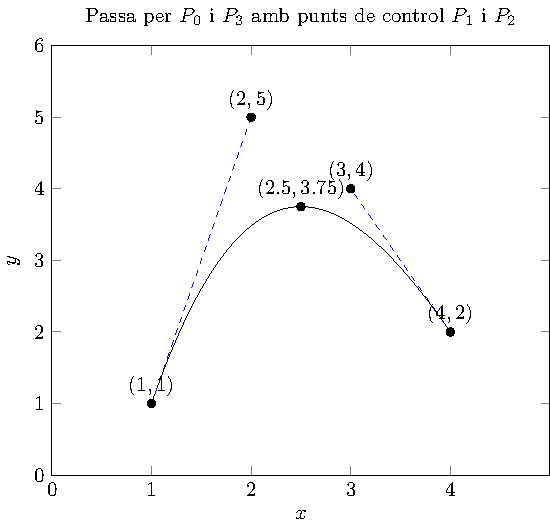
\includegraphics{../figures/interpolaciobeziers2.pdf}
  \end{center}

\end{enumerate}